%\documentclass[11pt,a4paper,twocolumn]{elsarticle}
%\documentclass[preprint,12pt]{elsarticle}

%% Use the option review to obtain double line spacing
%% \documentclass[preprint,review,12pt]{elsarticle}

%% Use the options 1p,twocolumn; 3p; 3p,twocolumn; 5p; or 5p,twocolumn
%% for a journal layout:
%% \documentclass[final,1p,times]{elsarticle}
%% \documentclass[final,1p,times,twocolumn]{elsarticle}
%% \documentclass[final,3p,times]{elsarticle}
\documentclass[final,3p,times,twocolumn]{elsarticle}
%% \documentclass[final,5p,times]{elsarticle}
%% \documentclass[final,5p,times,twocolumn]{elsarticle}

\usepackage[latin1]{inputenc}
\usepackage{amsmath}
\usepackage{amsfonts}
\usepackage{amssymb}
\usepackage{graphicx}
%\usepackage{cite}
\usepackage[usenames,dvipsnames]{color}
\usepackage{draftwatermark} \SetWatermarkScale{5} \SetWatermarkLightness{0.95}
\journal{Nuclear Nuclear Fusion}
\begin{document}
%\maketitle
\begin{frontmatter}

\title{In-Situ Spatially Resolved Measurement of Boron Erosion and Deposition in the Alcator C-Mod Tokamak}
%% use optional labels to link authors explicitly to addresses:
%% \author[label1,label2]{<author name>}
%% \address[label1]{<address>}
%% \address[label2]{<address>}

\author{H.S. Barnard, Z.S. Hartwig, B.N. Sorbom, P.W.Stahle, D.G.Whyte}

%\abstract{The accelerator based in-situ materials serveilance diagnostic (AIMS) was recently installed in 2012 to demonstrate the novel application of ion beam analysis to plasma materials interaction (PMI) science in the Alcator C-Mod Tokamak.  The first in-situ, spatially and temporally resolved measurements of material surface erosion and deposition are presented.  }

\begin{abstract}

The Accelerator Based In-situ Materials Surveillance (AIMS) diagnostic was recently developed to demonstrate the novel application of ion beam analysis (IBA) to in-vessel studies of plasma materials interaction in Alcator C-Mod. The AIMS diagnostic injects a 900 keV deuterium ion beam into the tokamak's vacuum vessel between plasma discharges while magnetic fields are used to steer the ion beam to plasma facing component (PFC) surfaces. Spectroscopic analysis of neutrons and gamma rays from the induced nuclear reactions provides a quantitative, spatially resolved map of the PFC surface composition that includes boron (B) and deuterium (D) content. Since AIMS is sensitive to low-Z elements and C-Mod regularly boronizes PFCs, the evolution of B and D on PFCs can be used to directly study erosion, deposition, and fuel retention in response to plasma operations and wall condition processes. AIMS analysis of 18 lower single null I-mode discharges show a net boron deposition rate of $6\pm2$~nm/s on the inner wall while subsequent inner wall limited discharges and a disruption did not show significant changes in B. Measurements of D content showed relative changes of $>$2.5 following a similar trend. This suggests high D retention rates and net B deposition rates of $\sim$18 cm/year of plasma exposure are possible and depend strongly on the plasma conditions. Ex-situ IBA was also performed on the same PFCs after removal from C-Mod, successfully validating the AIMS technique. These IBA measurements also show that the B content on the inner wall varied toroidally and poloidally from 0-3000 nm, demonstrating the importance of the spatial resolution provided by AIMS and the sensitivity of PFCs to B-field alignment.
\end{abstract}

\begin{keyword}
%% keywords here, in the form: keyword \sep keyword

%% MSC codes here, in the form: \MSC code \sep code
%% or \MSC[2008] code \sep code (2000 is the default)
KEYWORDS
\end{keyword}

\end{frontmatter}

%==============================================================================
% Introduction
%==============================================================================

\section{Introduction}
\label{sec:Intro}

Plasma materials interactions (PMI) present one the most significant engineering challenges for reactor-scale fusion devices. PMI however are difficult to study in laboratory tokamaks because they typically operate in short pulses with varied plasma conditions and provide little or no access to plasma facing components (PFC) under normal operating conditions. Due to this experimental constraint, it is often impossible to correlate plasma conditions to the effects of PMI thus leaving the plasma's dynamic effects on materials in fusion devices severely understudied.  The recent development of the AIMS diagnostic \cite{RSIPaper} (section \ref{sec:AIMSOverview}), however, has shown that it is now possible to directly measure the retention of hydrogen isotopes from the plasma \cite{HartwigDRetention} and the erosion and deposition of low-Z materials (presented in the following sections). These measurements provide new insight into the timescales and spatial variation of PMI effects on PFCs. 

%==============================================================================
% Background on IBA and AIMS
%==============================================================================

\section{Ion beam analysis and AIMS}
\label{sec:AIMSOverview}

A variety of ion beam analysis (IBA) techniques are commonly used to perform \textit{ex-situ} analysis on PFCs after they are removed from the tokamak. IBA involves using ion beams to induce nuclear reactions, elastic collisions, or atomic excitations in materials.  Spectroscopic measurements of the reaction products are then used to identify and quantify isotopes in the material's surface. A comprehensive description of these established methods  can be found in \cite{tesmer1995handbook}.

These IBA techniques serve an important function for studying long term aggregate PMI effects on PFCs \cite{wright2011plasma} and were instrumental in validating the AIMS technique (section \ref{sec:Validation}). However, since there are only rare occasions when PFCs can be removed for analysis, IBA studies are typically limited to long term net effects of PMI, often over the course of hundreds to thousands of plasma discharges.  Since these timescales spanning months of an experimental campaign with varying plasma configurations, there is essentially no way to diagnose how one plasma configuration affects PFCs as compared to another.

\begin{figure}[h]
 \centering
%  \includegraphics[width=140mm]{figures/AIMS_Overview_Schematic.png}
  \includegraphics[width=\columnwidth]{figures/AIMS_Overview_Schematic_LineDrawing.pdf}
 \caption{Schematic of AIMS components.  AIMS utilizes a radio frequency quadrupole (RFQ) accelerator produce a 900 keV D$^+$ beam to induce nuclear reactions on the surface of plasma facing components (PFC). Spectroscopy of the resulting neutrons and gamma rays allow for the identification and quantification of isotopes on PFC surfaces. AIMS uses beam optics and toroidal field $B_\phi$ to steer the beam and achieve spatially resolved measurements.}
 \label{fig:AIMSOverviewSchematic0}
\end{figure}

A new diagnostic technique referred to as accelerator-based \textit{in-situ} materials surveillance (AIMS) was developed to simultaneously improve the spatial and temporal resolution of IBA measurements. AIMS utilizes a compact linear accelerator, gamma detectors, and neutron detectors to measure the evolution of PFC surface composition inside a magnetic confinement device. The technique is non-destructive to the PFCs, can access large fractions of the total PFC surface area, and is not disruptive to facility operations because it is designed to operate between plasma discharges. AIMS is essentially an IBA based in-situ diagnostic that is directly integrated with a tokamak. In addition, AIMS also provides spatially resolved measurements with approximately 2 cm spatial resolution on the shot-to-shot time scale by using the tokamak's magnetic field coils and DC supplies to steer and target the beam over a relatively large region of the plasma facing first wall \cite{RSIPaper}.  The development and implementation of the AIMS diagnostic, illustrated in figure \ref{fig:AIMSOverviewSchematic0}, was successfully implemented on Alcator C-Mod, making its first measurements during the 2012 experimental campaign. These measurements of boron erosion are presented and discussed in section~\ref{sec:Results}.

%==============================================================================
% Background on Boron and low Z erosion
%==============================================================================

\section{Wall conditioning and boron measurements}
\label{sec:BZNOverview}

High-Z refractory metal PFCs, particularly tungsten, are leading material choices for reactor PFCs. This is due to their low erosion, low tritium retention, favorable thermal properties, and robustness to neutron damage and activation. As a result, Alcator C-Mod uses almost entirely molybdenum PFCs -- a high-Z refractory metal with similar properties to W.  Despite the advantages of W and Mo, when high-Z elements enter the plasma energy confinement and plasma performance is degraded severely due to increased radiation from the high-Z impurities. %This tends to have strong negative impact on C-Mod plasma performance when operating with bare Mo PFCs, typically only achieving H-Mode plasmas with poor confinement $H_\mathrm{ITER,89} \sim 1$.  
%The impurity problems were successfully mitigated early on with the C-Mod boronization process. 
This issue is mitigated in C-Mod with the boronization process which involves plasma depositing boron on PFCs. The boron surface films tend to getter oxygen and are preferentially sputtered rather than the high-Z bulk of the PFCs, limiting the impurities to primarily low-Z boron. This results in significant improvement in plasma performance, often doubling the energy confinement time. When PFCs are boronized, the impurity radiation of the confined plasma drops substantially and the performance improves, essentially doubling energy confinement time, with $H_\mathrm{ITER,89}$ approaching 2. These coatings evolve on short $< 1$~sec timescales with regular plasma operations and on longer $>1$~hour timescales with plasma cleaning processes such as electron cyclotron discharge cleaning (ECDC) and glow discharge cleaning (GDC).

\subsection{Plasma conditioning and boronization}
Electron cyclotron discharge cleaning (ECDC) and boronization are the two most common plasma conditioning operations used in C-Mod to remove and add material on PFCs, respectively. ECDC is typically performed over several hours with a magnetized helium plasma that is heated at the electron cyclotron resonance and is used to to remove impurities from PFCs through sputtering. The resonance region is swept radially for uniform coverage by varying the B-Field (with typical parameters: frequency f = 2.45 GHz, B = 0.088 T at $R_o = 0.67$ m). Boronization is performed by a using the same plasma conditions except using a helium-diborane gas mixture (10\% B$_2$D$_6$, 90\% He) leading to net boron deposition across PFCs in the divertor. Glow discharge cleaning (GDC) using helium plasma generated by a high voltage electrode is used occasionally to remove impurities through sputtering, particularly following a vacuum break (NEED TO VERIFY THIS). In addition to C-Mod plasma discharges, all three of these techniques were used to following the C-Mod campaign to induce additional surface changes for observation with AIMS.

% The consistent use of boroniation means that there is 
\subsection{Boron measurements and PMI}
Boronization, ECDC, and GDC have all been empirically shown to improve plasma performance through their respective mechanisms, however, there is still very little quantitative understanding of how the boron on surfaces evolve with plasma exposure and wall conditioning. For example, the improvement in performance due to boronization degrades with plasma exposure yet boron remains on most surfaces according ex-situ measurements. This indicates that boron erosion and high-Z injection is a highly localized phenomenon with a significant impact on performance \cite{WWoBoronization}. AIMS will therefore be instrumental in exploring these processes because of short timescale and spatially resolved capabilities. Furthermore, even though boronization is not necessarily feasible for long pulsed devices or reactors, the erosion and deposition of boron is important to study because it can serve as a proxy for high-Z erosion. It may also play a vital role in understanding erosion in reactors as well as the complex net transport of materials, localized impurity injection, fuel retention due to co-deposition, an many other consequences of PMI.

%(10\% B$_2$D$_6$, 90\% He) \cite{WWoBoronization}.
% (with typical parameters: field f = 2.45 GHz, B = 0.088 T at $R_o = 0.67$ m). (%10\% B$_2$D$_6$, 90\% He),


%because these regions lead to impurity injection in high performance tokamaks like C-Mod can identify the regions or plasma conditions that are responsible for the degraded performance.  Thus, measurements of boron can serve as a proxy for high-Z erosion and may play a vital role in understanding erosion in reactors as well as the complex net transport of materials throughout the the tokamak due to PMI.

%==============================================================================
% Overview of AIMS boron analysis 
%==============================================================================

\section{AIMS analysis of boron in Alcator C-Mod}

AIMS Measurements were made at four poloidal locations on the inner wall of Alcator C-Mod before, during, and after the last run day of the 2012 C-Mod campaign to observe the effects of plasma discharges. Subsequent measurements were taken during the months following the campaign to observe changes due to plasma conditioning operations that include boronization, electron cyclotron discharge cleaning (ECDC), and glow discharge cleaning (GDC).

%------------------------------------------------------------------------------
% Descrition of Geomentry 
\subsection{AIMS beam and detection geometry}

AIMS measurements were taken spanning the accessible beam steering range. The range was limited by the toroidal field power supplies available at the time ($B_\phi$ ranging 0 to 0.16~T on axis). The beam trajectories were calculated numerically to predict the location of the deuterium beam PFCs. A 6D envelope dynamics code was also developed and used to calculate the evolution of the beam's distribution to predict the beam spot-size when projected on analyzed region of the PFCs. This was necessary to determine the spatial resolution of the measurements. Further details of the simulation tools and methods developed for AIMS are described \cite{AIMSBeamSim}. The beam trajectories, target locations, and projected beam spots are shown in figure \ref{fig:TileMap0}.

\begin{figure}[!h]
 \centering
  \includegraphics[width=\columnwidth]{figures/Beam_Spots_Projected_on_Tiles.pdf}
 \caption{\small Top: A poloidal projection of deuteron beam trajectories are shown for four trajectories spanning the range of the AIMS measurements. These trajectories and locations correspond to toroidal beam steering fields $B_\phi$ = \{0.000, 0.0582, 0.1135, 0.1618\} Tesla (in order from top to bottom). Bottom: Tile map of the C-Mod inner wall and inner divertor between the B and A port regions. This mapping shows the locations of the PIGE and AIMS measurements on the plasma facing tiles. The blue, green, red, and cyan ellipses indicate the calculated location and projected beamspots for AIMS measurements based on beam modeling. The tiles highlighted in yellow were removed and PIGE analyzed following AIMS measurements.}
 \label{fig:TileMap0}
\end{figure}


%------------------------------------------------------------------------------
% Descrition of timeline 

\subsection{AIMS Timeline}

AIMS measurement were made in two session: during the last run day of the 2012 campaign (table~\ref{tab:CampaignTimeline}), then one month later between a series of plasma conditioning processes (table~\ref{tab:PostCampaignTimeline}) designed to add or remove boron. The run day included 18 lower single null (LSN) I-mode discharges. These were followed by inner wall limited (IWL) discharges intended to maximize heat and particle flux on the locations accessible AIMS on the inner wall with one discharge ending in a disruption. Inter-shot measurements were made at the $B_\phi = 0$~T location after the LSN, and between IWL discharges at only one location was possible because of the required $\sim$10 minute detector acquisition time.

%
\begin{table}
 \centering
 \begin{tabular}{ll}
  \hline
  & Run-day plasma/analysis \\ \hline \hline 
  (1)&\textbf{AIMS at 4 locations} \\
  &\textcolor{green}{18 lower single null shots}  \\
  (2)&\textbf{AIMS at 1 location} \\
  &\textcolor{red}{2 Inner wall limited shots} \\
  &\textcolor{red}{Inner wall limited disruption}\\
  (3)&\textbf{AIMS at 1 location} \\
  &\textcolor{red}{2 Inner wall limited shots} \\
  (4)&\textbf{AIMS at 4 locations} \\
  &\textit{End of plasma shots} \\ \hline
 \end{tabular}
  \caption{Timeline of AIMS measurement during the 2012 C-Mod campaign.  Processes that are expected to cause net erosion are colored in red. The effect of the lower single null discharges on the inner wall is unknown and is shown in green.}  
  \label{tab:CampaignTimeline}
\end{table}
  
In the months following the campaign two boronizations were performed to measure the amount of deposited boron during the boronization process. This was followed by two electron cyclotron discharge cleanings (ECDC) and a glow discharge cleaning (GDC) to observe boron erosion and/or the effects of these standard wall conditioning techniques. A timeline for these measurements and plasma wall conditioning operations is given in table~\ref{tab:PostCampaignTimeline}. 

\begin{table}
 \centering
 \begin{tabular}{ll}\hline
  &Plasma conditioning/analysis \\ \hline \hline
  (4)&\textbf{AIMS at 4 locations} \\
  &\textcolor{blue}{Standard Overnight BZN}  \\
  &\textcolor{blue}{Inner Wall Overnight BZN}  \\
  (5)&\textbf{AIMS at 4 locations}  \\
  &\textcolor{red}{ECDC plasma}  \\
  (6)&\textbf{AIMS at 4 locations} \\
  &\textcolor{red}{ECDC plasma}  \\
  (7)&\textbf{AIMS at 4 locations} \\
  &\textcolor{red}{GDC Plasma}  \\
  (8)&\textbf{AIMS at 4 locations} \\
  &\textit{Vacuum break, 64 tiles removed} \\
  (9)&\textbf{Ion beam analysis of 64 tiles} \\ \hline
 \end{tabular}
 \caption{Timeline of post-campaign AIMS measurement and wall conditioning. Red and blue represent processes that are expected to cause net erosion and deposition of boron, respectively.}
 \label{tab:PostCampaignTimeline}
\end{table}

%------------------------------------------------------------------------------
% Description of Spectroscopy Techniques

\subsection{AIMS Gamma Spectroscopy}

For AIMS, gamma spectroscopy of photons from deuterium induced reactions is the primary method for quantifying the boron on PFCs. Gamma spectra taken with a lanthanum bromide (LaBr$_3$) detector were analyzed to observe the 953 keV peak in the spectrum from the $^{11}$B($d,p\gamma$)$^{12}$B reaction, the most prominent deuterium-boron reaction in the $<$~1~MeV D$^+$ beam energy range. A typical spectrum from the LaBr$_3$ detector used for AIMS is shown in figure \ref{fig:ZoomedInAIMSPhotopeak}. The integrated counts in the 953 keV peak is used to determine the boron areal density on the surface

\begin{figure}[!h]
 \centering
  \includegraphics[width=\columnwidth]{figures/AIMS_Gamma_Spectrum_Highlighted.pdf}
 \caption{Close up view of a 953 keV photopeak in an AIMS gamma spectrum from the $^{11}$B($d,p\gamma$)$^{12}$B.  Poisson error bars show that each bin within the peak is statistically significant and distinguishable from background.  The other notable feature, the 847 keV gammas from inelastic neutron-scattering off iron is also visible and distinguishable from the 953 keV photopeak.}
 \label{fig:ZoomedInAIMSPhotopeak}
\end{figure}

Quantitative measurements with AIMS are challenging because the beam geometry and detection geometry change with measurement location, affecting the absolute calibration of each measurement. These experimental factors are seen in the integral equation \ref{eq:YieldEXP} which relates the ion beam, target, and detection parameters to the number of gamma photons that are counted by the detector $N_\mathrm{\gamma,det}$. The first integral giving number of ions incident on the target $N_\mathrm{ion}$ is given equation \ref{eq:IonCurrent}) and the second integral giving the total gamma yield (photons per incident ion) from the reaction (equation \ref{eq:GammaYieldInegral})

\begin{equation}
%N_\mathrm{\gamma,det} = \frac{\eta(\chi_\mathrm{\gamma d}) \:\Omega_\mathrm{det}}{\cos(\theta_\mathrm{\gamma n})} 
%\int_0^{t_\mathrm{max}} \frac{I_\mathrm{b}}{e\:Z}\;dt\;
%\int_0^{ x_\mathrm{max}} n_B(x)\:\sigma(E(x))\;dx 
%N_\mathrm{\gamma,det} = \frac{\eta(\chi_\mathrm{\gamma d}) \:\Omega_\mathrm{det}}{\cos(\theta_\mathrm{\gamma n})} %\; N_\mathrm{ion}(t)\;
%\int_0^{ x_\mathrm{max}} n_B(x)\:\sigma(E(x))\;dx 
N_\mathrm{\gamma,det} = \frac{\eta(\chi_\mathrm{\gamma d}) \:\Omega_\mathrm{det}(\chi_\mathrm{\gamma d},L)}{\cos(\theta_\mathrm{\gamma n})} \; N_\mathrm{ion}(t)\;Y_\mathrm{\gamma}(n(x),E)
\label{eq:YieldEXP}
\end{equation}

\begin{equation}
N_\mathrm{ion}(t_\mathrm{det}) = \int_0^{t_\mathrm{det}} \frac{I_\mathrm{beam}(t)}{e\:z_\mathrm{ion}} \; dt
\label{eq:IonCurrent}
\end{equation}

\begin{equation}
Y_\mathrm{\gamma}(n(x),E) = \int_0^{ x_\mathrm{max}} n_B(x)\:\sigma(E(x))\;dx
\label{eq:GammaYieldInegral}
\end{equation}

The detector efficiency $\eta$ and the detector solid angle, 


integrals account for effects of beam and detection geometry these parameters are calculated numerically through simulation techniques described in \cite{AIMSBeamSim}. These parameters include the geometric parameters defined graphically in figure \ref{fig:AIMSDetectionCoordinates}. The absolute detector efficiency $\eta(\chi_\mathrm{\gamma d})$ and the detector solid angle $\Omega_\mathrm{det}$ are also necessary to make quantitative measurements. 

The first integral, where $I_{b}$ is the is the beam current and $eZ$ is the ion charge, is measured directly with a toroidal ferrite core transformer encircling the beamline near the injection flange.  The integral of $I_\mathrm{b}$ gives the total charge $Q_\mathrm{b}$ that is incident on the target PFC. 

The second integral is independent of the experiment geometry and depends only on the beam energy $E$ and the composition of the PFC surface; the boron density profile $n_\mathrm{B}(x)$ and reaction cross section $\sigma(E)$. Since boron is the dominant low Z element in C-Mod and exists as a solid surface layer of $\sim 1$~$\mu$m thickness, all of the boron content is assumed to be in a solid, uniform layer of boron of thickness $x_\mathrm{B}$ with a density of $n_B$. With this assumption, the second integral was solved numerically using nuclear cross section data \cite{sziki2006gamma} and ion stopping data \cite{SRIM} to give the total gamma yield per incident ion $Y_\mathrm{\gamma}$ as a function of boron thickness $x_\mathrm{B}$. The calculated $Y_\mathrm{\gamma}(x_\mathrm{B})$ is related directly to the yield measured in the detector $N_\mathrm{\gamma,det}$ with equation \ref{eq:YieldEXPsimple} which is inverted to give the thickness of boron and thus the areal density observed in the measurement.  

\begin{equation}
%N_\mathrm{\gamma,det} = \left( \frac{Q_\mathrm{b}}{e\:Z\:}\right) \left(\frac{\eta(\chi_\mathrm{\gamma d}) \:\Omega_\mathrm{det}}{\cos(\theta_\mathrm{\gamma n})}\right) Y_\mathrm{\gamma}(x_B)
Y_\mathrm{\gamma}(x_B)  =  \left(\frac{\cos(\theta_\mathrm{\gamma n})}{\eta(\chi_\mathrm{\gamma d}) \:\Omega_\mathrm{det}}\right) \frac{N_\mathrm{\gamma,det}}{N_\mathrm{ion}}
\label{eq:YieldEXPsimple}
\end{equation}


\begin{figure}[!h]
  \centering
  \includegraphics[width=\columnwidth]{figures/AIMSDetectionCoordinates.pdf}
  \caption{Graphical definitions for detector geometry.}
  \label{fig:AIMSDetectionCoordinates}
\end{figure}

The detection geometry changes as the beam position moves so the solid angle $\Omega_\mathrm{det}$ subtended by the detector must be properly accounted for in the analysis. Since the detector area $\Delta A_{det} \ll r^2$, where $r$ the distance from the target to the detector, the detection efficiency $\eta_{det}$ and solid angle $\Omega_{det}$ are given by equation \ref{eq:SolidAngleDet}.

MENTION NOT ALL GAMMA MEASUREMENTS WORKED

\subsection{AIMS Neutron Analysis}

Energy resolved measurement of the neutrons were taken concurrently with the gamma measurements using an EJ301 liquid organic scintillator coupled to a photomultiplier tube residing outside of the C-Mod field coils.  The details of the neutron detection equipment and theory are given in~\cite{HartwigThesis}.  Unlike the gamma spectra, these neutron spectra do not contain distinct features that identify boron. However, the high energy neutrons in the spectra are the result of down-scattering of neutrons produced by only boron reactions and are therefore indicative of the boron content. 

\begin{figure}[h!]
 \centering
  \includegraphics[width=\columnwidth]{figures/BoronIntegrationPlot.pdf}
 \caption{Relative measurements of boron are made from the AIMS neutron spectra by integrating the high energy portion of the spectrum shown in blue, corresponding to neutron from the $^{10}$B($d,n$)$^{11}$C and $^{11}$B($d,n$)$^{12}$C reactions.  The `channels' on the spectrum correspond to the binning of charge output from the detector which is related to scintillator light output and is a non-linear function of energy.  The region of integration shown from 1.8 - 2.5 corresponds a region of in which only neutrons from boron are energetically allowed~\cite{HartwigThesis}.}
 \label{fig:BoronNeutronSpectrum}
\end{figure}

The correlation between neutron and gamma measurements is expected because only boron and deuterium have neutron producing reactions shown in table \ref{tab:NeutronReactions} with boron reaction producing substantially higher energy neutrons. Whereas the other elements present in PFCs in C-Mod include only molybdenum, tungsten, and oxygen which do not produce neutrons from $< 1$~MeV deuterons.

\begin{table}[h]
\centering
 \begin{tabular}{lr}
  \hline Neutron Reactions & Q [keV]  \\ \hline \hline 
  $^\mathrm{10}$B$(d,n)^\mathrm{11}$C & 6464.804 \\
  $^\mathrm{11}$B$(d,n)^\mathrm{12}$C & 13732.283  \\
  $^\mathrm{11}$B$(d,n\: 2\alpha )^\mathrm{4}$He & 6457.542  \\
  $^\mathrm{11}$B$(d,n\: \alpha )^\mathrm{8}$Be & 6365.701 \\
  $^\mathrm{\;\;2}$H$(d,n)^\mathrm{3}$He & 3268.914 \\
  \hline
 \end{tabular}
\caption{900 keV deuteron induced neutron-producing reactions and their Q-values for low-Z isotopes on C-Mod PFCs.}
\label{tab:NeutronReactions}
\end{table}

% &   $^\mathrm{\;\;2}$H$(d,n)^\mathrm{3}$He & 3268.914

Empirical evidence of this correlation is shown in figure \ref{fig:AIMSNeutronsGammaCorrelation}.  For each AIMS measurement location and AIMS run where valid gamma and neutron data were available, the relationship between gamma counts $N_\gamma$ and neutron counts $N_n$ were compared where each point represents an AIMS measurement where $N_n$ and $N_g$ were measured simultaneously with the same target, beam current, and acquisition time.

\begin{figure}[h]
 \centering
  \includegraphics[width=\columnwidth]{figures/AIMS_Neutron_vs_Gamma_Correlation_Measured_LinearFit.pdf}
 \caption{Measured correlation between neutron $N_n$ and gamma $N_\gamma$ counts from AIMS measurement at four locations. Each point represents an AIMS measurement where $N_n$ and $N_\gamma$ were measured simultaneously with the same target, beam current, and acquisition time.  A linear fit is drawn for data sets that show a statically significant correlation.}
 \label{fig:AIMSNeutronsGammaCorrelation}
\end{figure}

The relationship between the neutrons counts $N_n$ and gamma counts $N_\gamma$ shows that, for the zero field case and the 0.058 T case, a statistically significant correlation between between the two detection techniques appears to be linear, tracking a 50\% change in boron induced counts.  This confirms the proportionality relationship $N_n \propto N_\gamma$.  For the other two target locations with steering fields, fewer gamma points were available, and the counting uncertainty in the photopeaks is relatively large.  %This made it more difficult to conclusively establish the proportionality between the $N_n$ and $N_\gamma$ measurements, although within the statistical uncertainty, the results do not disagree with the proportionality. 
Though these data are insufficient to show a similar trend, the physics is essentially identical between each location, only differing in beam and detection geometry.  There is also no physical reason to expect that another element to be present at only specific locations which could contribute to the neutron continuum.  It is therefore likely that a proportionality relationship exist for each of the four locations.

%From studying the results from these four locations in figure~\ref{fig:AIMSNeutronsGammaCorrelation}, it is also clear that the proportionality of the measurements between $N_n$ and $N_\gamma$ does not remain the same between locations.  This is not unexpected and is likely due to a variety of factors including the angular dependence of the cross sections, detection geometry, complex neutron scattering geometry, and differing mean free paths of neutrons and gammas in the presence of obstructions in the detection geometry.   

As a result of establishing the relationship between $N_n$ and $N_\gamma$, this integration of the high energy neutron counts can thus be used to provide a relative measurement of boron content that can be absolutely calibrated from the gamma photopeaks to allow trends in the boron evolution to be studied in the absence of a contiguous set of gamma measurements. These results are shown in section \ref{sec:Results}.

\section{AIMS Results and Discussion}
\label{sec:Results}

The quantitative AIMS measurements of boron from the 953~keV gamma photopeaks were combined with the measurements of high energy scattered neutrons to construct a complete time history of areal density of boron present on the plasma facing molybdenum tiles. Th

Outline of Error analysis: 
\begin{itemize}
\item The wide rectangle surrounding each point represents the error bars associated with measurement technique.  These include the Poisson error from particle detection and current integration and other experimental uncertainties. 
\item For the neutron measurements, the narrow error bars represent error with respect to the absolute quantity calibration which is based on a least squares fit to the overlapping gamma measurements.
\item For the PIGE measurements, the narrow error bars represent the uncertainty in the comparison since PIGE measurements are made at a single location in the center of each tile while AIMS measurements are made over the surface area of roughly one tile. This uncertainty estimate was made based on the average variation in boron thickness within a single tile.  
\item The PIGE comparison error is larger for $B_\phi=0.058$~T as also substantially larger than the $B_\phi=0.000$~T case because the beam target spans the corner of 3 tiles. 
\end{itemize}



Results Results Results Results Results Results Results Results Results Results Results Results Results Results Results Results Results Results Results Results Results Results Results Results Results 



\begin{figure}[h]
 \centering
  \includegraphics[width=\columnwidth]{figures/AIMSBoronHistoryNoField.pdf}
 \caption{...................}
 \label{fig:BoronTimeHistoryB0}
\end{figure}

\begin{figure}[h]
 \centering
  \includegraphics[width=\columnwidth]{figures/AIMSBoronResults4Locations.pdf}
 \caption{...................}
 \label{fig:BoronResults4Locations}
\end{figure}

\section{Ion Beam Analysis for AIMS Validation}
\label{sec:Validation}
Ex-situ ion beam analysis was performed on the PFCs that were studied with AIMS to provide an independent validation of the AIMS measurements. Particle induced gamma emission (PIGE) analysis, a well established quantitative IBA technique \cite{HaroldsThesisPHD,XMIBA,IBA7}, was performed on 64 plasma facing molybdenum tiles that were removed from C-Mod inner wall after the completion of the AIMS measurements. Analysis was performed with a 2 MeV external proton beam using the tandem accelerator at the CLASS facility \cite{wright2011plasma}. A 3 inch diameter sodium iodide (NaI) detector was used to detect the induced 432 keV gammas from the $^\mathrm{10}$B$(p,\alpha\gamma)^\mathrm{7}$Be to quantify the boron the PFCs. The setup used, the locations of the overlapping PIGE and AIMS, and boron measurements are shown in figure \ref{fig:ExSituAnalysis}.


\begin{figure}[h!]
 \centering
  \includegraphics[width=\columnwidth]{figures/ExSituAnalysisCombined.pdf}
 \caption{Top: Photo of tiles analyzed using ex-situ PIGE. Outlines of the beam spots used for PIGE analysis are shown in red. Beamspot from AIMS measurements for $B_\phi=0$~T and $B_\phi = 0.0582$~T are shown in blue. Bottom: Boron areal density measured with PIGE analysis is represented as boron thickness assuming a solid boron surface layer. AIMS beamspots are show in blue.}
 \label{fig:ExSituAnalysis}
\end{figure}

\section{Summary and Conclusions}

The AIMS diagnostic was successfully implemented on Alcator C-Mod yielding the first spatial resolved and quantitative in-situ measurements of boron in a tokamak.  By combining AIMS neutron and gamma measurements, time resolved and spatially resolved measurements of boron were made, spanning the entire AIMS run campaign which included lower single null plasma shots, inboard limited plasma shots, a disruption, and C-Mod wall conditioning procedures.  These measurements demonstrated the capability if AIMS to perform inter-shot measurements at a single location and spatially resolved measurements on over longer timescales (with great potential for improved timescales and resolution).  This demonstration showed the first in-situ measurements of surfaces in a magnetic fusion device with spatial and temporal resolution which constitutes a major step forward in fusion PMI science.

An external ion beam system was also implemented to perform ex-situ ion beam analysis (IBA) on large components removed from Alcator C-Mod.  This system was used to perform particle induced gamma emission (PIGE), a well established IBA technique, on tile modules to validate the AIMS technique.  From these external PIGE measurements, a spatially resolved map of boron areal density was constructed for a section of C-Mod inner wall tiles that overlapped with the AIMS measurement locations.  These measurements showed the complexity of the poloidal and toroidal variation of boron areal density between PFC tiles on the inner wall ranging from 0 to 3$\mu$m of boron.  Using these well characterized ex-situ measurements to corroborate the in-situ measurements, AIMS showed reasonable agreement with PIGE, thus validating the quantitative boron detection capability of the AIMS technique.

\bibliographystyle{plain}
\bibliography{AIMSBoronAnalysis.bib}

\end{document}
